\documentclass{report}
\usepackage[utf8]{inputenc}
\usepackage[portuges]{babel}
\usepackage{fullpage}
\usepackage{graphicx}
\usepackage{tikz}
\usepackage{titlesec}
\usetikzlibrary{er,positioning}
\renewcommand{\baselinestretch}{0.5}


\author{Bruna Meneguzzi \\ Caio Calisto Gaede Hirakawa \\ Eduardo Freire de Carvalho Lima \\ Jiang Zhi \\ Matheus Santos Conceição}
\title{Exercício-Programa 1: Base de dados}
\begin{document}
\maketitle
\tableofcontents
\chapter{Parte I: Entendimento e validação do modelo}
Nesse exercício-programa iremos modelar o banco de dados para um sistema de gestão de grades curriculares da USP, a partir dos dois modelos conceituais oferecidos. No capítulo atual iremos discutir quais serão os benefícios e os malefícios de cada um desses dois modelos conceituais e tentar criar um novo modelo conceitual a partir deles.

Alguns pontos que sabemos é que nesse banco de dados utilizamos uma estrutura de persistência, ou seja, os dados somente podem ser acrescentados e além disso não podem ser modificados. Essa falta de variabilidade de dados faz com que a modelagem do banco de dados fique mais complicada, criando uma necessidade de um planejamento antecipado para alguns sistemas que modificam de ano para ano seus dados, como os cursos obrigatórios, onde os cursos necessários podem mudar, os cursos lecionados, onde os cursos disponíveis podem mudar, o novo sistema de trilhas, onde os requerimentos para cumprir a trilha podem mudar.

Para os cursos obrigatórios e o novo sistema de trilhas podemos usar um sistema externo para colocar as matérias feitas e verificar quais são os requisitos que precisam ser cumpridos. Após a verificação podemos marcar no banco de dados quais foram as matérias cumpridas e se terminamos os cursos obrigatórios e/ou completamos uma trilha, evitando criar um banco de dados para marcar os requisitos da trilha e das obrigatórias de cada ano dentro do banco. Mas devido a ausência desse sistema externo, precisamos criar um módulo para colocar os currículos.

O sistema de cursos lecionados pode ser feito facilmente, pois acrescentamos os dados ao decorrer das aulas lecionadas pelos  professor sobre a disciplina.

Inicialmente foi proposto o modelo MER-X 1, onde vemos que existe um trecho onde definimos a grade como obrigatória ou optativa, essa trecho pode ser transformado em informação da entidade Disciplina. Como mostrado no modelo MER-X 2 onde o banco de dados fica mais compacto.

Assim, utilizaremos o modelo MER-X 2 com algumas modificações para a modelagem do nosso banco de dados.


\chapter{Parte II: Modelo Conceitual e suas classes abstratas}

\section{Entidades}
\subsection{Pessoa:}
  A entidade regular Pessoa é uma entidade chave para nosso modelo e é nela que armazenaremos todos os dados das instâncias de cada uma das pessoas da USP presentes na nossa base de dados, seja ela Aluno, Professor ou Administrador.
  
  Segundo nosso modelo, cada instância de Pessoa será composta por seu número USP, que será utilizado como chave primária, seu CPF, que será utilizado como chave secundária, seu nome, e-mail, sexo, data de nascimento e endereço, que será um atributo composto de logradouro, número, complemento, bairro, município, unidade federativa e CEP.
  
  O listing abaixo traz um exemplo da estrutura da entidade:
\begin{itemize}
  \item Número USP  (Chave primária)
  \item CPF (Chave secundária)
  \item Nome
  \item E-mail
  \item Sexo
  \item Data de Nascimento
  \item Endereço:
  \begin{itemize}
    \item Logradouro
    \item Número
    \item Complemento
    \item Bairro
    \item Município
    \item Unidade Federativa
    \item CEP
  \end{itemize}
\end{itemize}
\begin{tikzpicture}
  \node[entity] (node1) {Pessoa}
  child [grow=-130,level distance=3cm]{node[attribute] {pe\_Email}}
  child [grow=-30,level distance=3cm]{node[attribute] {pe\_Nome}}
  child [grow=-55,level distance=3cm]{node[attribute] {\underline{pe\_NUSP}}}
  child [grow=+30,level distance=3cm]{node[attribute] {pe\_DataNasc}}
  child [grow=+60,level distance=3cm]{node[attribute] {pe\_Sexo}}
  child [grow=-95,level distance=3cm]{node[attribute] {\underline{\underline{pe\_CPF}}}}
  child [grow=0,level distance=3cm]{node[attribute] {pe\_Endereço}
      child [grow=40,level distance=3cm]{node[attribute] {pe\_Numero}}
      child [grow=16,level distance=4cm]{node[attribute] {pe\_Complemento}}
      child [grow=4,level distance=3.5cm]{node[attribute] {pe\_Bairro}}
      child [grow=-10,level distance=4cm]{node[attribute] {pe\_Municipio}}
      child [grow=-25,level distance=4cm]{node[attribute] {pe\_UF}}
      child [grow=-60,level distance=3cm]{node[attribute] {pe\_CEP}}
    };
\end{tikzpicture}

\paragraph{Restrições de Domínio:}

\begin{itemize}
  \item \textbf{pe\_NUSP:} Chave primária da entidade Pessoa. Sequência de 6 a 9 dígitos, englobando todos os números USP conhecidos e mais um dígito para quando os dígitos disponíveis não forem suficientes. Não pode ser nulo.
  \item \textbf{pe\_CPF:} Chave secundária da entidade Pessoa. Sequência de 11 dígitos que passe pelas regras de validação da Receita Federal:
  \begin{itemize}
    \item verificação do primeiro dígito
    \item verificação de segundo dígito
    \item verificação de dígitos iguais
  \end{itemize}
  Não pode ser nulo.
  \item \textbf{pe\_Nome:} Sequência de letras maiúsculas e minúsculas, apóstrofe, hífen e espaço. No mínimo de 5 e máximo de 80 caracteres. Não pode ser nulo.
  \item \textbf{pe\_Email:} Sequência de 1 a 80 caracteres alfanuméricos e caracteres especiais \begin{verbatim}(!#$%&'*+-/=?^_`{|}~.) \end{verbatim} seguidos de um @, seguido de mais uma sequência de 1 a 80 caracteres alfanuméricos e caracteres especiais \begin{verbatim}(!#$%&'*+-/=?^_`{|}~.)
  \end{verbatim} .
  Não pode ser nulo.
  \item \textbf{pe\_DataNasc:} no formato data dd/mm/aaaa. Não pode ser nulo.
  \item \textbf{pe\_Sexo:} M, F ou N, representando Sexo Masculino, Feminino ou Não declarado respectivamente.
  \item \textbf{pe\_Endereco:}
  \begin{itemize}
    \item \textbf{pe\_Logradouro:} Sequência de caracteres alfanuméricos, apóstrofe, hífen e espaço. No mínimo de 4 e máximo de 80 caracteres. Não pode ser nulo.
    \item \textbf{pe\_Numero}: Sequência de 1 a 10 caracteres alfanuméricos e espaço, com o intuito de permitir escrever "sem número". Não pode ser nulo.
    \item \textbf{pe\_Complemento:} Sequência de caracteres alfanuméricos, apóstrofe, hífen e espaço. No mínimo de 4 e máximo de 80 caracteres. Pode ser nulo.
    \item \textbf{pe\_Bairro:} Sequência de caracteres alfanuméricos, apóstrofe, hífen e espaço. No mínimo de 4 e máximo de 80 caracteres. Não pode ser nulo.
    \item \textbf{pe\_Municipio:} Complemento Logradouro: Sequência de caracteres alfanuméricos, apóstrofe, hífen e espaço. No mínimo de 4 e máximo de 80 caracteres. Não pode ser nulo.
    \item \textbf{pe\_UF:} Complemento Logradouro: Sequência de caracteres alfanuméricos, apóstrofe, hífen e espaço. No mínimo de 4 e máximo de 80 caracteres. Não pode ser nulo.
    \item \textbf{pe\_CEP:} Sequência de 5 dígitos, seguido de um hífen, seguidos de mais três dígitos. Não pode ser nulo.
    \end{itemize}
\end{itemize}


O listing traz um exemplo de possíveis tuplas a serem inseridas em Pessoa, no formato (NUSP, CPF, Nome, Email, Sexo, DataNasc, Logradouro, Numero, Complemento, Bairro, Municipio, UF, CEP):

\begin{itemize}
  \item 7777777; 003.939.708-41; Juca Araujo; juca@usp.br; M; 01/04/1999; Avenida A, 10, null, Butanta, Sao Paulo, SP, 10.200-100
  \item 7777888;076.713.684-58; Celia; celia@usp.br; F; 02/03/2000; Avenida B, 11, apto 11, Pinheiros, Sao Paulo, SP, 01.500-250

\end{itemize}
\subsection{Aluno:}
  A entidade regular Aluno é uma entidade chave para nosso modelo e é nela que armazenaremos todos os dados das instâncias de cada um dos alunos da USP presentes na nossa base de dados.
  
  Segundo nosso modelo, cada instância de Aluno será composta por sua Data de Ingresso, o Código do Curso a qual ele pertence e a quantidade de Créditos Acumulados por ele até o momento da consulta, que será um atributo composto por créditos referentes a disciplinas Obrigatórios, Eletivas e Livres.
  
  O listing abaixo traz um exemplo da estrutura da entidade:
\begin{itemize}
  \item Data de Ingresso
  \item Código do Curso
  \item Créditos acumulados
  \begin{itemize}
    \item Obrigatórios
    \item Optativos Eletivos
    \item Optativos Livres
  \end{itemize}
\end{itemize}
\begin{tikzpicture}
  \node[entity] (node1) {Aluno}
  child [grow=+10,level distance=3cm]{node[attribute] {al\_CodCurso}}
  child [grow=-90,level distance=1cm]{node[attribute] {al\_DataIngresso}}
  child [grow=-10,level distance=3cm]{node[attribute] {al\_Creditos}
    child [grow=-20,level distance=3cm]{node[attribute] {al\_Obrigatorios}}
    child [grow=-70,level distance=2cm]{node[attribute] {al\_Eletivos}}
    child [grow=-135,level distance=2cm]{node[attribute] {al\_Livres}}
  };
  
\end{tikzpicture}
\paragraph{Restrições de Domínio:}
\begin{itemize}
  \item \textbf{Data de Ingresso:} Data no formato dd/mm/aaaa. Não pode ser nulo.
  \item \textbf{Código do Curso:} Números entre 1 e +infinito. Não pode ser nulo.
  \item \textbf{Créditos acumulados:}
  \begin{itemize}
    \item \textbf{Obrigatórios:} inteiro entre 0 e +infinito. Não pode ser nulo.
    \item \textbf{Optativos Eletivos:} inteiro entre 0 e +infinito. Não pode ser nulo.
    \item \textbf{Optativos Livres:} inteiro entre 0 e +infinito. Não pode ser nulo.
  \end{itemize}
\end{itemize}

O listing traz um exemplo de possíveis tuplas a serem inseridas em Aluno, no formato (DataIngr, CodCurso, Obrigatorios, Eletivos, Livres):

\begin{itemize}
  \item 01/02/2016; 42; 0, 0, 0
  \item 03/02/2017; 15; 0, 0, 0
\end{itemize}

A inserção de um aluno no banco de dados sempre acarretará que ele entre com 0 créditos e, para alterá-lo no decorrer de seu período na USP, um procedure será feito.
\subsection{Professor:}
  A entidade regular Professor é uma entidade chave para nosso modelo e é nela que armazenaremos todos os dados das instâncias de cada um dos professores da USP presentes na nossa base de dados.
  
  Segundo nosso modelo, cada instância de Professor será composta por seu Departamento, Data de Admissão e Área de atuação, que será um atributo multivalorado.
  
  O listing abaixo traz um exemplo da estrutura da entidade:
\begin{itemize}
  \item Departamento
  \item Data de Admissão
  \item Área de Atuação
\end{itemize}
\begin{tikzpicture}
  \node[entity] (node1) {Professor}
    child [grow=-30,level distance=3cm]{node[attribute] {pr\_Departamento}}
  child [grow=+0,level distance=3cm]{node[attribute] {pr\_Area}}
    child [grow=-80,level distance=2.5cm]{node[attribute] {pr\_DataAdmissao}};
  \draw[black] (3, 0) ellipse (0.9 and 0.3);
\end{tikzpicture}
\paragraph{Restrições de Domínio:}
\begin{itemize}
  \item \textbf{pr\_Departamento:} Sequência de caracteres alfanuméricos, apóstrofe, hífen e espaço. No mínimo de 4 e máximo de 80 caracteres. Não pode ser nulo.
  \item \textbf{pr\_DataAdmissao:} Data no formato dd/mm/aaaa. Não pode ser nulo.
  \item \textbf{pr\_Area:} Sequência de caracteres alfanuméricos, apóstrofe, hífen e espaço. No mínimo de 4 e máximo de 80 caracteres. Não pode ser nulo.
\end{itemize}

O listing traz um exemplo de possíveis tuplas a serem inseridas em Professor no formato (Departamento, DataAdmissao, Area):

\begin{itemize}
  \item IME; 01/02/1985; Software. 
  \item FMU; 05/03/2000; Neurologia, Clinico Geral
  \item BIO; 10/01/1992; Zoologia
\end{itemize}

\subsection{Administrador:}
A entidade regular Administrador é uma entidade chave para nosso modelo e é nela que armazenaremos todos os dados das instâncias de cada um dos administradores dos cursos da USP presentes na nossa base de dados.
  
  Segundo nosso modelo, cada instância de Administrador será composta por sua Data de Inicio do mandato e Data de Término, este último podendo ser nulo, indicando que o mandato ainda está em vigência.
    
  O listing abaixo traz um exemplo da estrutura da entidade:
\begin{itemize}
  \item Data de Início da Gestão
  \item Data de Término da Gestão
\end{itemize}
\begin{tikzpicture}
  \node[entity] (node1) {Administrador}
  child [grow=-30,level distance=3cm]{node[attribute] {adm\_DataIni}}
  child [grow=-80,level distance=2.5cm]{node[attribute] {adm\_DataTerm}};
\end{tikzpicture}
\paragraph{Restrições de Domínio:}
\begin{itemize}
  \item \textbf{adm\_DataInicio:} Data no formato dd/mm/aaaa. Não pode ser nulo.
  \item \textbf{adm\_DataTermino:} Data no formato dd/mm/aaaa.
\end{itemize}
O listing traz um exemplo de possíveis tuplas a serem inseridas em Administrador no formato (DataIni, DataTerm):

\begin{itemize}
  \item 01/01/2010; 31/12/2015. 
  \item 01/01/2016; null.
\end{itemize}
\subsection{Disciplina:}
A entidade regular Disciplina é uma entidade chave para nosso modelo e é nela que armazenaremos todos os dados das instâncias de cada um das discilinas da USP presentes na nossa base de dados.
  
  Segundo nosso modelo, cada instância de Disciplina será composta por seu Nome, Código, que será sua chave primária, Departamento a que pertence, Ementa, Descrição do que é lecionado nela, Pré-Requisitos, um atributo multivalorado, Período Ideal e quantidade de créditos que ela fornece.
    
  O listing abaixo traz um exemplo da estrutura da entidade:
\begin{itemize}
  \item Nome
  \item Código (Chave Primária)
  \item Departamento
  \item Ementa
  \item Descrição
  \item Pré-requisitos
  \item Período ideal
  \item Créditos:
  \begin{itemize}
    \item Aula
    \item Trabalho
    \end{itemize}
\end{itemize}
\begin{tikzpicture}
  \node[entity] (node1) {Disciplina}
    child [grow=45,level distance=3cm]{node[attribute] {dis\_Nome}}
    child [grow=25,level distance=3cm]{node[attribute] {\underline{dis\_Codigo}}}
    child [grow=130,level distance=2cm]{node[attribute] {dis\_Departamento}}
    child [grow=-30,level distance=3.5cm]{node[attribute] {dis\_Ementa}}
    child [grow=0,level distance=3.5cm]{node[attribute] {dis\_Pre-requisitos}}
    child [grow=-60,level distance=3cm]{node[attribute] {dis\_Descrição}}
    child [grow=-130,level distance=4cm]{node[attribute] {dis\_PeríodoIdeal}}
    child [grow=180,level distance=4cm]{node[attribute] {dis\_Creditos}
      child [grow=-150,level distance=2cm]{node[attribute] {dis\_Aula}}
      child [grow=-60,level distance=1.5cm]{node[attribute] {dis\_Trabalho}}
    };
  \draw[black] (3.5, 0) ellipse (1.9 and 0.3);
\end{tikzpicture}
\paragraph{Restrições de Domínio:}
\begin{itemize}
  \item \textbf{dis\_Nome:} Sequência de caracteres alfanuméricos, apóstrofe, hífen e espaço. No mínimo de 4 e máximo de 80 caracteres. Não pode ser nulo.
  \item \textbf{dis\_Codigo:}  Sequência de caracteres alfanuméricos. No mínimo de 4 e máximo de 9 caracteres. Não pode ser nulo.
  \item \textbf{dis\_Depart:} Sequência de caracteres alfanuméricos, apóstrofe, hífen e espaço. No mínimo de 4 e máximo de 80 caracteres. Não pode ser nulo.
  \item \textbf{dis\_Ementa:} Sequência de caracteres alfanuméricos, apóstrofe, hífen e espaço. No mínimo de 4 e máximo de 80 caracteres. Não pode ser nulo.
  \item \textbf{dis\_Descricao:} Sequência de caracteres UTF-8. Mínimo de 4 e máximo de 1000 caracteres. Não pode ser nulo.
  \item \textbf{dis\_PreRequis:} Sequencia de caracteres alfanuméricos. No mínimo de 4 de 80 caracteres. 
  \item \textbf{dis\_PerIdeal:}  Numéro inteiro entre 1 e 12.
  \item \textbf{dis\_Aula:} Inteiro positivo entre 1 e 50.
  \item \textbf{dis\_Trabalho:} Inteiro positivo entre 1 e 50.
\end{itemize}

O listing traz um exemplo de possíveis tuplas a serem inseridas em Disciplina no formato (Nome, Codigo, Depart, Ementa, Descricao, PreRequis, PerIdeal, Aula, Trabalho):

\begin{itemize}
  \item Introdução a Computação; MAC110; MAC; Variáveis, Condicionais, Loops; Conceitos básicos de Programação; null; 1; 4, 2.
  \item Analise de Algoritmo; MAC425; MAC; Complexidade, Programação Dinâmica, Gulosos; Analisar custo de tempo e espaço extra em algoritmos clássicos; MAC323, MAC215; 4, 0.
\end{itemize}
%%%%%%%%%%%%%%%%%%%%%%%%%%%%%%%%%%%%%%%%%%%%%%%%%%%%%%%%%%%%%%%%%%%%%%
%\paragraph{Especialização da Disciplina:}
%\begin{itemize}
% \item \textbf{Obrigatória:}
%     \begin{itemize}
%         \item \textbf{teste:}
%     \end{itemize}
%     \begin{tikzpicture}
%         \node[entity] (node1) {Obrigatória};
%     \end{tikzpicture}
%     \paragraph{Restrições de Domínio:}
%     \begin{itemize}
%       \item \textbf{teste2:}
%     \end{itemize}
%     
% \item \textbf{Eletiva:}
% \item \textbf{Livre:} 
%\end{itemize}
%
%----------------------------------------------------------------------------------------------------------------------------------------------------------------------------------------
%Acho que não precisa colocar Obrigatoria/eletiva/livre dentro de Disciplina. Declara como Entidade né? Mesmo sendo especialização
%eu acho que sim
%----------------------------------------------------------------------------------------------------------------------------------------------------------------------------------------
%
%%%%%%%%%%%%%%%%%%%%%%%%%%%%%%%%%%%%%%%%%%%%%%%%%%%%%%%%%%%%%%%%%%%%%%
%%%%%%%%%%%%%%%%%%%%%%%%%%%%%%%%%%%%%%%%%%%%%%%
% parei de inserir as restrições aqui, mas mesmo restrições anteriores devem
% precisar de uma revisão, principalmente no número max e min de carateres
%%%%%%%%%%%%%%%%%%%%%%%%%%%%%%%%%%%%%%%%%%%%%%%%%%%%%%%%%%%%%
\subsection{Currículo:}
A entidade regular Currículo é uma entidade chave para nosso modelo e é nela que armazenaremos todos os dados das instâncias de cada um currículos dos cursos da USP presentes na nossa base de dados.
  
  Segundo nosso modelo, cada instância de Currículo será composta por seu Ano de Inicio, Ano de Fim, este último podendo ser nulo, indicando que o currículo ainda está em vigência para um certo Curso, Unidade e Curso a qual o currículo pertence.
    
  O listing abaixo traz um exemplo da estrutura da entidade:
\begin{itemize}
  \item Ano de Início (Chave primária)
   \item Ano de Fim
   \item Unidade
   \item Curso
\end{itemize}
\begin{tikzpicture}
  \node[entity] (node1) {Currículo}
    child [grow=0,level distance=3cm]{node[attribute] {\underline{cur\_AnoIni}}}
  child [grow=-25,level distance=3.5cm]{node[attribute] {cur\_Unidade}}
  child [grow=-165,level distance=3.5cm]{node[attribute] {cur\_Curso}}
  child [grow=-90,level distance=1.5cm]{node[attribute] {cur\_AnoFim}};
\end{tikzpicture}
\paragraph{Restrições de Domínio:}
\begin{itemize}
  \item \textbf{cur\_AnoIni:} Número inteiro de 4 dígitos entre 1500 e +infinito.
   \item \textbf{cur\_AnoFim:} Número inteiro de 4 dígitos entre 1500 e +infinito.
   \item \textbf{cur\_Curso:} Sequência de caracteres. No mínimo de 2 até 80 caracteres.
   \item \textbf{cur\_Unidade:} Sequência de caracteres. No mínimo de 2 até 80 caracteres.
\end{itemize}
O listing traz um exemplo de possíveis tuplas a serem inseridas em Currículo no formato (AnoIni, AnoFim, Curso, Unidade):

\begin{itemize}
  \item 01/01/2000; 31/12/2016; 42; IME. 
  \item 01/01/2017; null; 42; IME
\end{itemize}
%%%%%%%%%%%%%%%%%%%%%%%%INICIO INICIO INICIO INICIO INICIO%%%%%%%%%%%%%%%%%%%%%%%%%%%%%%%%%%%%%%%%
\iffalse
\subsection{Obrigatória:} 
\begin{itemize}
  \item 
\end{itemize}
\begin{tikzpicture}
  \node[entity] (node1) {Obrigatoria};
\end{tikzpicture}
\subsection{Optativa:}  
\begin{itemize}
 \item
\end{itemize}
\begin{tikzpicture}
 \node[entity] (node1) {Optativa};
\end{tikzpicture}
\subsection{Eletiva:}
\begin{itemize}
  \item
\end{itemize}
\begin{tikzpicture}
  \node[entity] (node1) {Eletiva};
\end{tikzpicture}
\subsection{Livre:}
\begin{itemize}
  \item
\end{itemize}
\begin{tikzpicture}
  \node[entity] (node1) {Livre};
\end{tikzpicture}
\fi
%%%%%%%%%%%%%%%%%%%%%%%%%%%%FIM FIM FIM FIM FIM FIM%%%%%%%%%%%%%%%%%%%%%%%%%%%%%%%%%%%%%%
\subsection{Módulo:}
A entidade regular Módulo é uma entidade chave para nosso modelo e é nela que armazenaremos todos os dados das instâncias de cada um dos módulos existentes dos cursos da USP presentes na nossa base de dados.
  
  Segundo nosso modelo, cada instância de Módulo será composta por seu Nome e Código, este sendo sua chave primária.
    
  O listing abaixo traz um exemplo da estrutura da entidade:
\begin{itemize}
  \item Nome
  \item Código (Chave primária)
\end{itemize}
\begin{tikzpicture}
  \node[entity] (node1) {Modulo}
    child [grow=-30,level distance=3cm]{node[attribute] {mod\_Nome}}
    child [grow=-80,level distance=3cm]{node[attribute] {\underline{mod\_Codigo}}};
\end{tikzpicture}
\paragraph{Restrições de Domínio:}
\begin{itemize}
  \item \textbf{mod\_Nome:} Sequência de caracteres alfanuméricos, apóstrofe, hífen e espaço. No mínimo de 4 e máximo de 80 caracteres. Não pode ser nulo.
  \item \textbf{mod\_Codigo:} Sequência de caracteres numéricos. No mínimo de 1 e máximo de 9 caracteres. Não pode ser nulo.
\end{itemize}
O listing traz um exemplo de possíveis tuplas a serem inseridas em Módulo no formato (Nome, Codigo):

\begin{itemize}
  \item Matematica Discreta I; 1. 
  \item Algoritmos 2; 5.
\end{itemize}
\subsection{Trilha:}
A entidade regular Trilha é uma entidade chave para nosso modelo e é nela que armazenaremos todos os dados das instâncias de cada uma das trilhas dos cursos da USP presentes na nossa base de dados.
  
  Segundo nosso modelo, cada instância de Trilha será composta por seu Nome e Código, este último sendo sua chave primária.
    
  O listing abaixo traz um exemplo da estrutura da entidade:
\begin{itemize}
  \item Nome
  \item Código (Chave primária)
\end{itemize}
\begin{tikzpicture}
  \node[entity] (node1) {Trilha}
    child [grow=-30,level distance=3cm]{node[attribute] {tr\_Nome}}
    child [grow=-80,level distance=3cm]{node[attribute] {\underline{tr\_Codigo}}};
\end{tikzpicture}
\paragraph{Restrições de Domínio:}
\begin{itemize}
  \item \textbf{tr\_Nome:} Sequência de caracteres alfanuméricos, apóstrofe, hífen e espaço. No mínimo de 4 e máximo de 80 caracteres. Não pode ser nulo.
  \item \textbf{tr\_Codigo:} Sequência de caracteres alfanuméricos. No mínimo de 4 e máximo de 9 caracteres. Não pode ser nulo.
\end{itemize}
O listing traz um exemplo de possíveis tuplas a serem inseridas em Trilha no formato (Nome, Codigo):

\begin{itemize}
  \item Inteligência Artificial; 10. 
  \item Teoria da Computação; 3.
\end{itemize}
\subsection{Usuário:}
  A entidade regular Usuário é uma entidade chave para nosso modelo e é nela que armazenaremos todos os dados das instâncias de cada um dos Usuários da nossa plataforma presentes na nossa base de dados.
  
  Segundo nosso modelo, cada instância de Usuário será composta por seu Login, este sendo sua chave primária, sua Senha e seu Username.
    
  O listing abaixo traz um exemplo da estrutura da entidade:
\begin{itemize}
  \item Login (Chave primária)
  \item Senha
  \item Username
\end{itemize}
\begin{tikzpicture}
  \node[entity] (node1) {Usuario}
    child [grow=-10,level distance=3cm]{node[attribute] {\underline{us\_login}}}
    child [grow=-30,level distance=3cm]{node[attribute] {us\_senha}}
    child [grow=-60,level distance=3cm]{node[attribute] {us\_username}};
\end{tikzpicture}
\paragraph{Restrições de Domínio:}
\begin{itemize}
  \item \textbf{us\_Login:} Sequência de caracteres alfanuméricos. No mínimo de 6 até 80 caracteres. Não pode ser nulo.
  \item \textbf{us\_Senha:}  Sequência de caracteres alfanuméricos. No mínimo de 6 até 80 caracteres. Não pode ser nulo.
  \item \textbf{us\_Username:} Sequência de caracteres alfanuméricos, separados ou não pode espaço. No mínimo de 6 até 80 caracteres. Não pode ser nulo.
\end{itemize}
O listing traz um exemplo de possíveis tuplas a serem inseridas em Usuário no formato (Login, Senha, Username):

\begin{itemize}
  \item anabeatriz2007; 123456; Ana Bia. 
  \item marcelinho2000; 102030; Marcelo Silva
\end{itemize}
\subsection{Perfil:}
  A entidade regular Perfil é uma entidade chave para nosso modelo e é nela que armazenaremos todos os dados das instâncias de cada um dos Perfis da nossa plataforma presentes na nossa base de dados.
  
  Segundo nosso modelo, cada instância de Perfil será composta apenas por seu Tipo, que será sua chave primária.
    
  O listing abaixo traz um exemplo da estrutura da entidade:
\begin{itemize}
  \item Tipo
\end{itemize}
\begin{tikzpicture}
  \node[entity] (node1) {Perfil}
    child [grow=-90,level distance=1.5cm]{node[attribute] {\underline{pr\_Tipo}}};
\end{tikzpicture}
\paragraph{Restrições de Domínio:}
\begin{itemize}
  \item \textbf{pr\_Tipo:} Sequência de caracteres alfanuméricos. No mínimo de 4 e máximo de 80 caracteres. Não pode ser nulo.
\end{itemize}
O listing traz um exemplo de possíveis entradas a serem inseridas em Perfil no formato (Tipo):

\begin{itemize}
  \item Visitante
  \item Aluno Monitor.
\end{itemize}
\subsection{Serviço:}
  A entidade regular Serviço é uma entidade chave para nosso modelo e é nela que armazenaremos todos os dados das instâncias de cada um dos Serviços presentes na nossa base de dados.
  
  Segundo nosso modelo, cada instância de Serviço será composta por seu Nome, que será sua chave primária, e uma Descrição de cada um deles. 
    
  O listing abaixo traz um exemplo da estrutura da entidade:
\begin{itemize}
  \item Nome (Chave primário)
  \item Descrição
\end{itemize}
\begin{tikzpicture}
  \node[entity] (node1) {Serviço}
  child [grow=-90,level distance=1.5cm]{node[attribute] {\underline{ser\_Nome}}}
  child [grow=-20,level distance=3cm]{node[attribute] {ser\_Descrição}};
\end{tikzpicture}
\paragraph{Restrições de Domínio:}
\begin{itemize}
  \item \textbf{ser\_Nome:} Sequência de caracteres alfanuméricos. No mínimo de 4 e máximo de 80 caracteres. Não pode ser nulo.
    \item \textbf{ser\_Descrição:} Sequência de caracteres alfanuméricos. No mínimo de 4 e máximo de 80 caracteres. Não pode ser nulo.
\end{itemize}
O listing traz um exemplo de possíveis tuplas a serem inseridas em Serviços no formato (Nome, Descrição):

\begin{itemize}
  \item Alteração; Alterar atributos de entidades e relacionamentos do Banco de Dados
  \item Inserção; Inserir dados no Banco de Dados, como novos alunos e novas disciplinas.
\end{itemize}
\section{Agregados}
\subsection{Oferecimento:}
 O agregado Oferecimento é um agregado chave para nosso modelo e é nele que armazenaremos todos os dados das instâncias de cada um dos Oferecimentos presentes na nossa base de dados.
  
  Segundo nosso modelo, cada instância de Oferecimento será composta por sua Data de Inicio, que será sua chave primária, seu horário, atributo multivalorado, e a quantidade máxima de Vagas que o oferecimento suporta.
      
  O listing abaixo traz um exemplo da estrutura da entidade:
\begin{itemize}
  \item Data de Início (Chave Primária)
  \item Horário
  \item Vagas
\end{itemize}
\begin{tikzpicture}
  \node[entity] (node1) {Oferecimento}
    child [grow=-45,level distance=2.5cm]{node[attribute] {\underline{of\_DataInicio}}}
    child [grow=-90,level distance=3cm]{node[attribute] {of\_Horario}}
    child [grow=-0,level distance=3cm]{node[attribute] {of\_Vagas}};
  \draw[black] (0, -3) ellipse (1.15 and 0.25);
\end{tikzpicture}
\paragraph{Restrições de Domínio:}
\begin{itemize}
  \item \textbf{ser\_DataInicio:} Data no formato dd/mm/aaaa. Não pode ser nulo.
  \item \textbf{ser\_Horario:} Horário no formato "ddd hh:mm - hh:mm", no qual ddd = dia da semana, hh = hora (00-23) e mm=minutos (00-59). Não pode ser nulo.
  \item \textbf{ser\_Vagas:} Número inteiro entre 1 e +infinito. Não pode ser nulo.
\end{itemize}
O listing traz um exemplo de possíveis tuplas a serem inseridas em Oferecimento no formato (DataInicio, Horario, Vagas):

\begin{itemize}
  \item 01/02/2019; TER 08:00 - 09:40, QUI 10:00 - 11:40; 60. 
  \item 01/08/2019; SEG 10:00 - 11:40, QUA 08:00 - 09:40; 40.
\end{itemize}
%%%%%%%%%%%%%%%%%%%%%%%%%%%%%%%%%%%%%%%%%%%%%%%%%%%%%%%%%%%%%%%%%%%%%%%%%%
%         Relacionamentos (estou achando que não precisa dessa parte
%%%%%%%%%%%%%%%%%%%%%%%%%%%%%%%%%%%%%%%%%%%%%%%%%%%%%%%%%%%%%%%%%%%%%%%%%%%
\section{Relacionamentos}
\subsection{pe\_us:}
Não identificamos a necessidade deste relacionamento conter atributos, pois só importa o mapeamento entre as entidades Pessoa e Usuário.
\subsection{us\_pf:}
O relacionamento us\_pf é um relacionamento chave para nosso modelo e é nele que armazenaremos todos os dados das instâncias de cada usuário com o tipo de perfil que ele possui.
  
  Segundo nosso modelo, cada instância de us\_pf será composta pela Data de início de quando um usuário adquiriu aquele perfil e sua data de término. 
  
  O listing abaixo traz um exemplo da estrutura da entidade:
\begin{itemize}
  \item Data de início
  \item Data de término
\end{itemize}
\begin{tikzpicture}
  \node[relationship] (node1) {us\_pf}
    child [grow=-35,level distance=3cm]{node[attribute] {up\_DataIniPerf}}
    child [grow=-75,level distance=3cm]{node[attribute] {up\_DataTermPerf}};
\end{tikzpicture}
\paragraph{Restrições de Domínio:}
\begin{itemize}
  \item \textbf{up\_DataIniPerf:} Data no formato dd/mm/aaaa. Não pode ser nulo.
  \item \textbf{up\_DataTermPerf:} Data no formato dd/mm/aaaa. Não pode ser nulo.
\end{itemize}
O listing traz um exemplo de possíveis tuplas a serem inseridas em us\_pf no formato (DataIniPerf, DataTermPerf):

\begin{itemize}
  \item 01/02/2019; 30/06/2019.
  \item 01/08/2019; 31/12/2019.
\end{itemize}
 \subsection{pf\_se:}
Não identificamos a necessidade deste relacionamento conter atributos, pois só
 importa o mapeamento entre as entidades Perfil e Serviço.
\subsection{Cursa:}
O relacionamento Curso é um relacionamento chave para nosso modelo e é nele que armazenaremos todos os dados das instâncias de cada um dos alunos da USP que cursarem alguma disciplina presentes na nossa base de dados.
  
  Segundo nosso modelo, cada instância de Cursa será composta pela Data de quando o Aluno cursou a Disciplina, que será a chave primária desse relacionamento, sua Frequência e Nota.
  
  O listing abaixo traz um exemplo da estrutura da entidade:
\begin{itemize}
  \item Data de Início (Chave primária)
  \item Frequência
  \item Nota
\end{itemize}
\begin{tikzpicture}
  \node[relationship] (node1) {Cursa}
        child [grow=0,level distance=3cm]{node[attribute] {\underline{c\_DataInic}}}
    child [grow=-35,level distance=3cm]{node[attribute] {c\_Nota}}
    child [grow=-60,level distance=3cm]{node[attribute] {c\_Frequencia}};
\end{tikzpicture}
\paragraph{Restrições de Domínio:}
\begin{itemize}
  \item \textbf{c\_DataIni:} Data no formato dd/mm/aaaa. Não pode ser nulo.
  \item \textbf{c\_Frequencia:} Número entre 0 e 100.
  \item \textbf{c\_Nota:} Número entre 0 e 10.
\end{itemize}
O listing traz um exemplo de possíveis tuplas a serem inseridas em Cursa no formato (DataIni, Frequência, Nota):

\begin{itemize}
  \item 01/02/2019; null; null.
  \item 01/08/2019; null; null.
\end{itemize}
Na inserção desse relacionamento no Banco de Dados, todo aluno começará com valores nulos de frequência de nota, implicando que ele está cursando aquela matéria. No momento em que ele realizou a matéria, um procedure será feito para alterar sua nota e frequência.
\subsection{Planeja:}
O relacionamento Planeja é um relacionamento chave para nosso modelo e é nele que armazenaremos todos os dados das instâncias de cada um dos alunos da USP e seu planejamento em cursar alguma disciplina presentes na nossa base de dados.
  
  Segundo nosso modelo, cada instância de Planeja será composta pela Data de quando o Aluno pretende cursar uma disciplina.
    
  O listing abaixo traz um exemplo da estrutura da entidade:
\begin{itemize}
  \item Data de Inscrição
\end{itemize}
\begin{tikzpicture}
  \node[relationship] (node1) {Planeja}
    child [grow=-45,level distance=3cm]{node[attribute] {pla\_DataInscri}};
\end{tikzpicture}
\paragraph{Restrições de Domínio:}
\begin{itemize}
  \item \textbf{pla\_DataInscri:} Data no formato dd/mm/aaaa. Não pode ser nulo.
\end{itemize}
O listing traz um exemplo de possíveis tuplas a serem inseridas em Planeja no formato (DataInscri):

\begin{itemize}
  \item 01/02/2019.
  \item 01/08/2019.
\end{itemize}
\subsection{Administra:}
O relacionamento Administra é um relacionamento chave para nosso modelo e é nele que armazenaremos todos os dados das instâncias de Administrador da USP e o início do seu mandato.
  
  Segundo nosso modelo, cada instância de Administra será composta pela Data de quando o Administrador começou a ser responsável por um curso.
    
  O listing abaixo traz um exemplo da estrutura da entidade:
\begin{itemize}
  \item Data de Início da Administração
\end{itemize}
\begin{tikzpicture}
  \node[relationship] (node1) {Administra}
    child [grow=-45,level distance=3cm]{node[attribute] {adm\_DataIniAdm}};
\end{tikzpicture}
\paragraph{Restrições de Domínio:}
\begin{itemize}
  \item \textbf{adm\_DataIniAdm:} Data no formato dd/mm/aaaa. Não pode ser nulo.
\end{itemize}
O listing traz um exemplo de possíveis tuplas a serem inseridas em Administra no formato (DataIniADM):

\begin{itemize}
  \item 01/02/2019.
  \item 01/08/2019.
\end{itemize}
\subsection{rel\_cur\_tri:}
 Não identificamos a necessidade deste relacionamento conter atributos, porque
 sua definição já está contida na relação Currículo.
\subsection{tr\_mo:}
 Não identificamos a necessidade deste relacionamento conter atributos, pois só
 importa o mapeamento entre as entidades Trilha e Módulo.
\subsection{rel\_dis\_mod:}
 Não identificamos a necessidade deste relacionamento conter atributos, pois só
 importa o mapeamento entre as entidades Disciplina e Módulo.
\subsection{Funcionalidades esperadas}
\begin{itemize}
  \item Permitir ao aluno planejar um cronograma de disciplinas segundo uma trilha
escolhida;
  \item Permitir o professor ao controle das disciplinas e dos eventuais oferecimentos dessas disciplinas;
  \item Permitir a administradores a gestão de
grades curriculares;
\end{itemize}


\break

\section {DER-X}
Como a modelagem do DER-X ficou muito extensa tivemos uma dificuldade de colocar essa modelagem dentro do pdf, mantendo as informações de forma legível.

\begin{figure}[!htb]
     \centering
     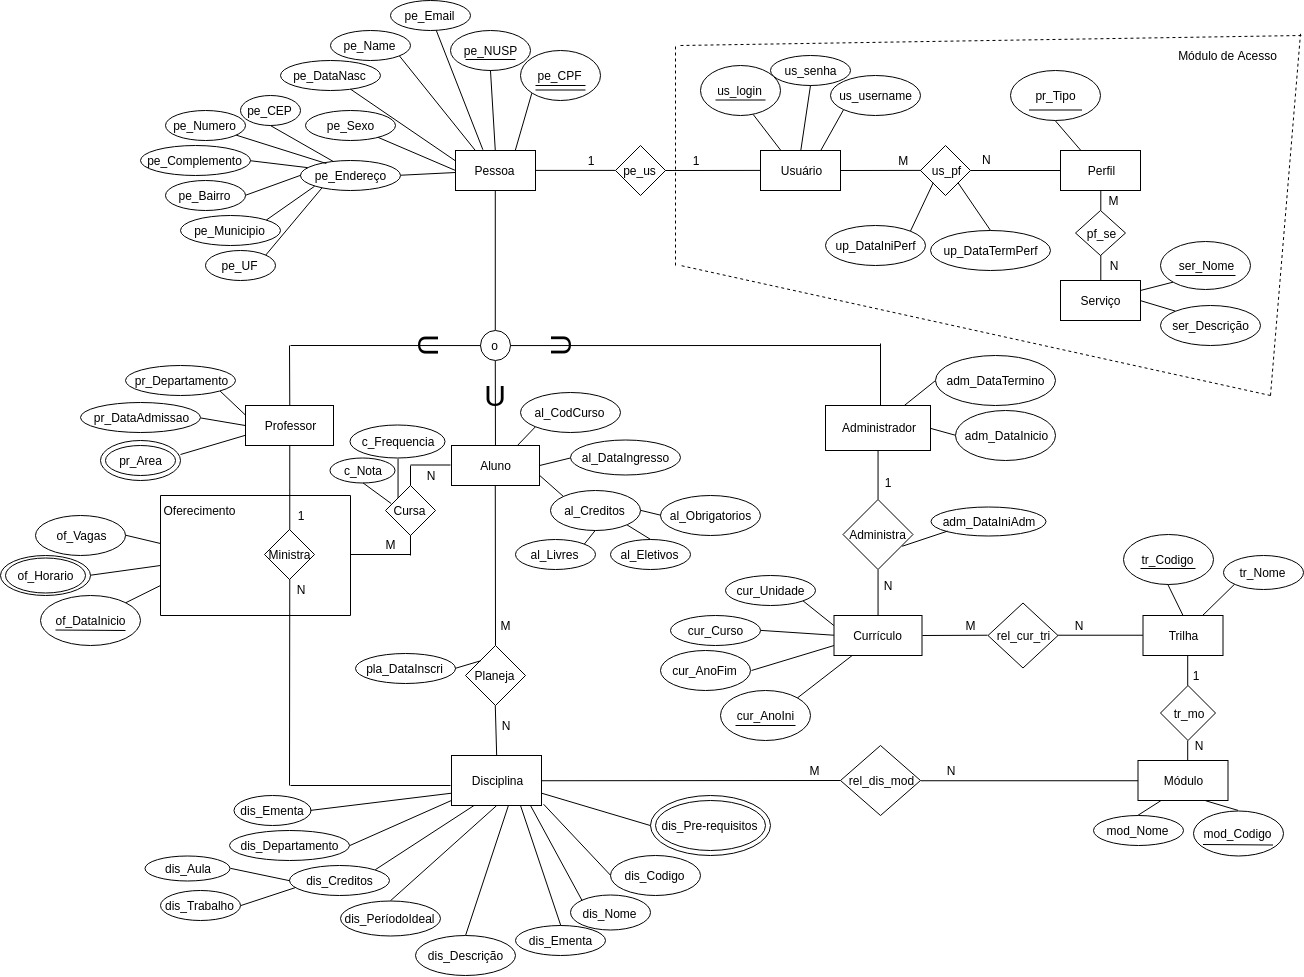
\includegraphics[scale=0.35]{imagens/EP1_DER.jpg}
     \caption{DER-X}
\end{figure}

Essa imagem, pode ser encontrada também na pasta imagens dentro do arquivo DER\_EP1.jpg


\chapter{Parte III: Modelo lógico e Físico}

\section{Modelo lógico}

O modelo conceitual pode ser transformado em lógico de maneira fácil, agora só precisamos saber quais são as chaves primárias e as chaves estrangeiras.

Para as chaves primárias podemos definir diretamente do modelo conceitual.

Para as chaves estrangeiras, precisamos observar para as relações, para as especializações, para a multivaloração.

Quando temos relações podemos criar uma chave estrangeira da tabela de relações para suas respectivas chaves primárias das entidades relacionadas.

Quando temos especialização, como aluno, professor e administrador, criamos a ligação dessas chave estrangeira dessas entidades para a entidade pessoal.

Quando temos uma multivaloração, criamos a ligação desses a entidade que contém esses múltiplos valores para a entidade principal que queremos achar.

Após finalizar esse processo, conseguimos um modelo lógico, mas esse modelo lógico ficou muito extenso e criamos um pdf que pode ser encontrado na pasta pdf no arquivo ModeloLogico.pdf.



\section{Modelo físico}
Nessa parte convertemos o modelo lógico em modelo físico, a partir das informações dentro das entidades e das suas chaves primárias e suas chaves estrangeiras criada no modelo lógico.

Algumas verificações de consistência de dados podem ser muito díficil de fazer internamente no banco de dados como saber se o e-mail é válido, então podemos fazer um checador de consistência externa no momento de inserir os dados e de periodos e periodos de tempo podemos checar a consistência interna do banco de dados.


\end{document}
